\documentclass[t]{beamer}
\usepackage[T1]{fontenc}
\usepackage[utf8]{inputenc}
\usepackage{lmodern}
\usepackage{amsmath}
\usepackage{amsfonts}
\usepackage{amssymb}
\usepackage{amsthm}
\usepackage{graphicx}
\usepackage{color}
\usepackage{xcolor}
\usepackage{url}
\usepackage{theorem}
\usepackage{textcomp}
\usepackage{listings}
\usepackage{hyperref}
\usepackage{glossaries}
\usepackage{parskip}
\usetheme{CambridgeUS}
\usepackage{pifont}
\usepackage{listings}
\usepackage{graphicx}
\graphicspath{ {./images/} }
\newcommand{\ite}{\item[\ding{118}]}
\title{Fair Division}
\author{Iniyan Joseph}
\date{ }
\setbeamertemplate{blocks}

\begin{document}

\begin{frame}
	\titlepage
\end{frame}

\begin{frame}{Dividing a cake}
	\begin{itemize}
		\item[\ding{118}] 
	\end{itemize}
\end{frame}

\begin{frame}{Dividing a cake}
	\begin{itemize}
		\item[\ding{118}] Imagine two people want to share this cake...
		\item[\ding{118}] But we have some problems
		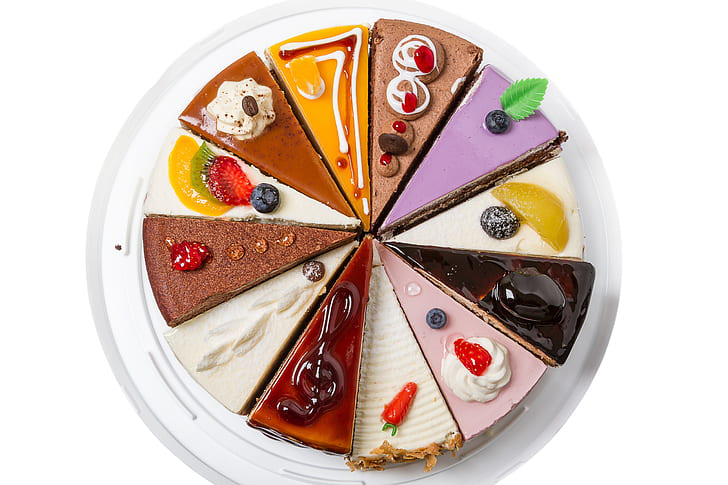
\includegraphics{cakeImage}[scale=1]
	\end{itemize}
\end{frame}

\begin{frame}{Dividing a cake}
	\begin{itemize}
		\ite This cake is complicated
		\ite Person 1 and Person 2 value different parts of the cake differently
		\ite Can we come up with an algorithm where both people are happy?
	\end{itemize}
\end{frame}
\begin{frame}{What is happiness anyways?}
	\begin{itemize}
		\ite Fairness
		\begin{itemize}
			\ite Every person believes that they received at least $\frac{1}{n}$ of the cake
			\ite $\mu_i(X_i)\geq \frac{1}{n}$
		\end{itemize}	
		\ite Envy-Freeness	
		\begin{itemize}
			\ite Every person believes that they received at least a good a piece of the cake as everyone else. 
			\ite $\forall_{i,j} \mu_i(X_i)\geq \mu_i(X_j)$
		\end{itemize}
		\ite Fair and envy-free divisions are always guaranteed to exist!
	\end{itemize}
\end{frame}
\begin{frame}{An ideal algorithm for n=2}
	\begin{itemize}
		\ite When n=2, an extremely simple algorithm exists
		\begin{itemize}
			\ite This solution is extremely old - it was first presented in the Torah
		\end{itemize}
		\ite One person can cut the cake, and the other person can choose their preferred piece
		\ite Therefore, this algorithm is called "Cut \& Choose"
	\end{itemize}
\end{frame}

\begin{frame}{Why does this work?}
	\begin{itemize}
		\ite The cutter gets exactly $\frac{1}{2}$ of the cake
		\ite The cutter knows that the other piece is also worth $\frac{1}{2}$ of the cake
		\ite The chooser gets the piece which they think is better
		\ite One of those pieces must be worth at least $\frac{1}{2}$ of the cake
		
		\ite The cutter is always incentivized to tell the truth - a concept in mechanism design called \textit{DISC (Dominant Strategy is Incentive Compatible)}
	\end{itemize}
\end{frame}

\begin{frame}{The need for generality}
	I'm a computer scientist! Don't just tell me for k people, tell me for \textit{n} people! \pause
	\begin{itemize}
		\ite Sadly, the envy-free problem is extremely non-trivial to generalize...
		\ite So let's first focus on fairness, which can be both tractable straightforward.
	\end{itemize}
	For n people, there are many algorithms for fair division
\end{frame}

\begin{frame}{Banach-Knaster Last Diminisher}
	\begin{itemize}
		\ite Banach-Knaster was the first proposed solution for fairness
		\ite for i = 1...n-1
		\ite Person i cuts $\frac{1}{n}$ of the cake and passes it to person i+1
		\ite Person i+1 cuts if they believe that the piece is $> \frac{1}{n}$ of the cake, then passes to person i+2, etc.
		\ite The last person to cut the cake now believes that the piece is worth $\frac{1}{n}$ of the cake, and 
		they may take the piece.
	\end{itemize}
\end{frame}

\begin{frame}{The price of lying}
	\begin{itemize}
		\ite If someone wants to lie, they do so at significant risk.
		\ite The only way they can lie is to not cut when they believe the piece of cake is worth $> \frac{1}{n}$. 
		
		\ite To make it clear why this doesn't work, let's show an extreme example
		\begin{itemize}
			\ite Person 1 cuts 98\% of the cake, with the goal of taking it for themselves.
			\ite After passing the cake around, the last diminisher has only cut the piece down to 97\% of the value of the cake!
			\ite Because Person 1 is not the last diminisher, they must continue playing, however they cannot receive more than 3\% of the cake.
		\end{itemize}
	\end{itemize}
\end{frame}

\begin{frame}{A $\sigma$-algebra of crumbs}
	We want to measure the number of cuts needed to cut the cake
	\begin{itemize}
		\ite In the worst case, all people cut at every turn.
		\ite First n people cut, then one player drops out
		\ite Then n-1 people cut, then n-2 people, etc.
		\ite Thus, the number of cuts needed is $\sum\limits_{i=1}^{n}i = \frac{n \ast (n+1)}{2} = O(n^2)$
		\ite In the best case, the first cutter is also the last diminisher so n cuts are sufficient.
	\end{itemize}
\end{frame}

\begin{frame}{Dubins-Spanier Moving Knife}
	\begin{itemize}
		\ite Here we can see another style of fair cake cutting solutions.
		\ite Rather than having many cuts, a "moving knife" can be used to allocate chunks of cake.
		\begin{itemize}
			\ite A knife moves over the cake continuously from one side to the opposite side (for example from left to right)
			\ite When a person thinks that the portion remaining from the starting side/previous cut is worth $\frac{1}{n}$, then they may say "Cut", and they will take the portion on the left side.
		\end{itemize}
	\end{itemize}
\end{frame}

\begin{frame}{Does this work?}
	\begin{itemize}
		\ite This works, because the same person who said "Cut" at any given point would have been the last diminisher in in the Banach-Knaster Last Diminisher Method.
		\ite On a surface level, this seems to take n-1 cuts, but this is incorrect. Instead, it takes an infinite number of cuts perpendicular to the direction of movement.
	\end{itemize}
\end{frame}
\end{document}